\section{Introduction}\label{sec:intro}
Over the past decades, the rise of JavaScript as the de facto
language for web development has expanded its reach to diverse fields.
Node.js~\cite{nodejs} supports server-side programming, React
Native~\cite{react-native} and Electron~\cite{electron} produce cross-platform
applications, and Moddable~\cite{moddable} and Espruino~\cite{espruino}
provide JavaScript environments in micro-controllers for IoT.  Such wide prevalent
uses place JavaScript at \#7 in the TIOBE Programming Community
index\footnote{https://www.tiobe.com/tiobe-index/}.  Thus, researchers have
developed static analyzers such as JSAI~\cite{jsai}, TAJS~\cite{tajs},
WALA~\cite{wala}, and SAFE~\cite{safe,safe2} to understand behaviors of
JavaScript programs and to detect their bugs in a sound manner.

However, static analysis of real-world JavaScript programs suffers from immensely
functional and dynamic features of JavaScript such as callback
functions, first-class property names, and dynamic code generation.
While they provide flexibility in software development, it is
challenging to statically analyze such features.  To overcome these problems,
researchers have proposed several analysis techniques: advanced string
domains~\cite{string, regex, combining-string}, loop sensitivity~\cite{lsaECOOP,
lsaSPE}, analysis based on property relations~\cite{correlation, weaklyAPLAS,
weaklySPE, value-partitioning}, and on-demand backward
analysis~\cite{value-refinement}.

At the same time, various JavaScript host environments require excessive
manual modeling of their behaviors for static analysis.  Because built-in functions and
host-dependent functions are implemented in native language like C and
C++ instead of JavaScript, their code is \textit{opaque} during static
analysis.  Thus, static analyzers often model their behaviors
manually, which is error-prone, tedious, and labor-intensive.
While several researchers have proposed automatic modeling
techniques~\cite{safewapi, model-ts}, since they utilize only type
information, they generate imprecise modeling compared with the manual approach.

\begin{figure}[t]
  \centering
  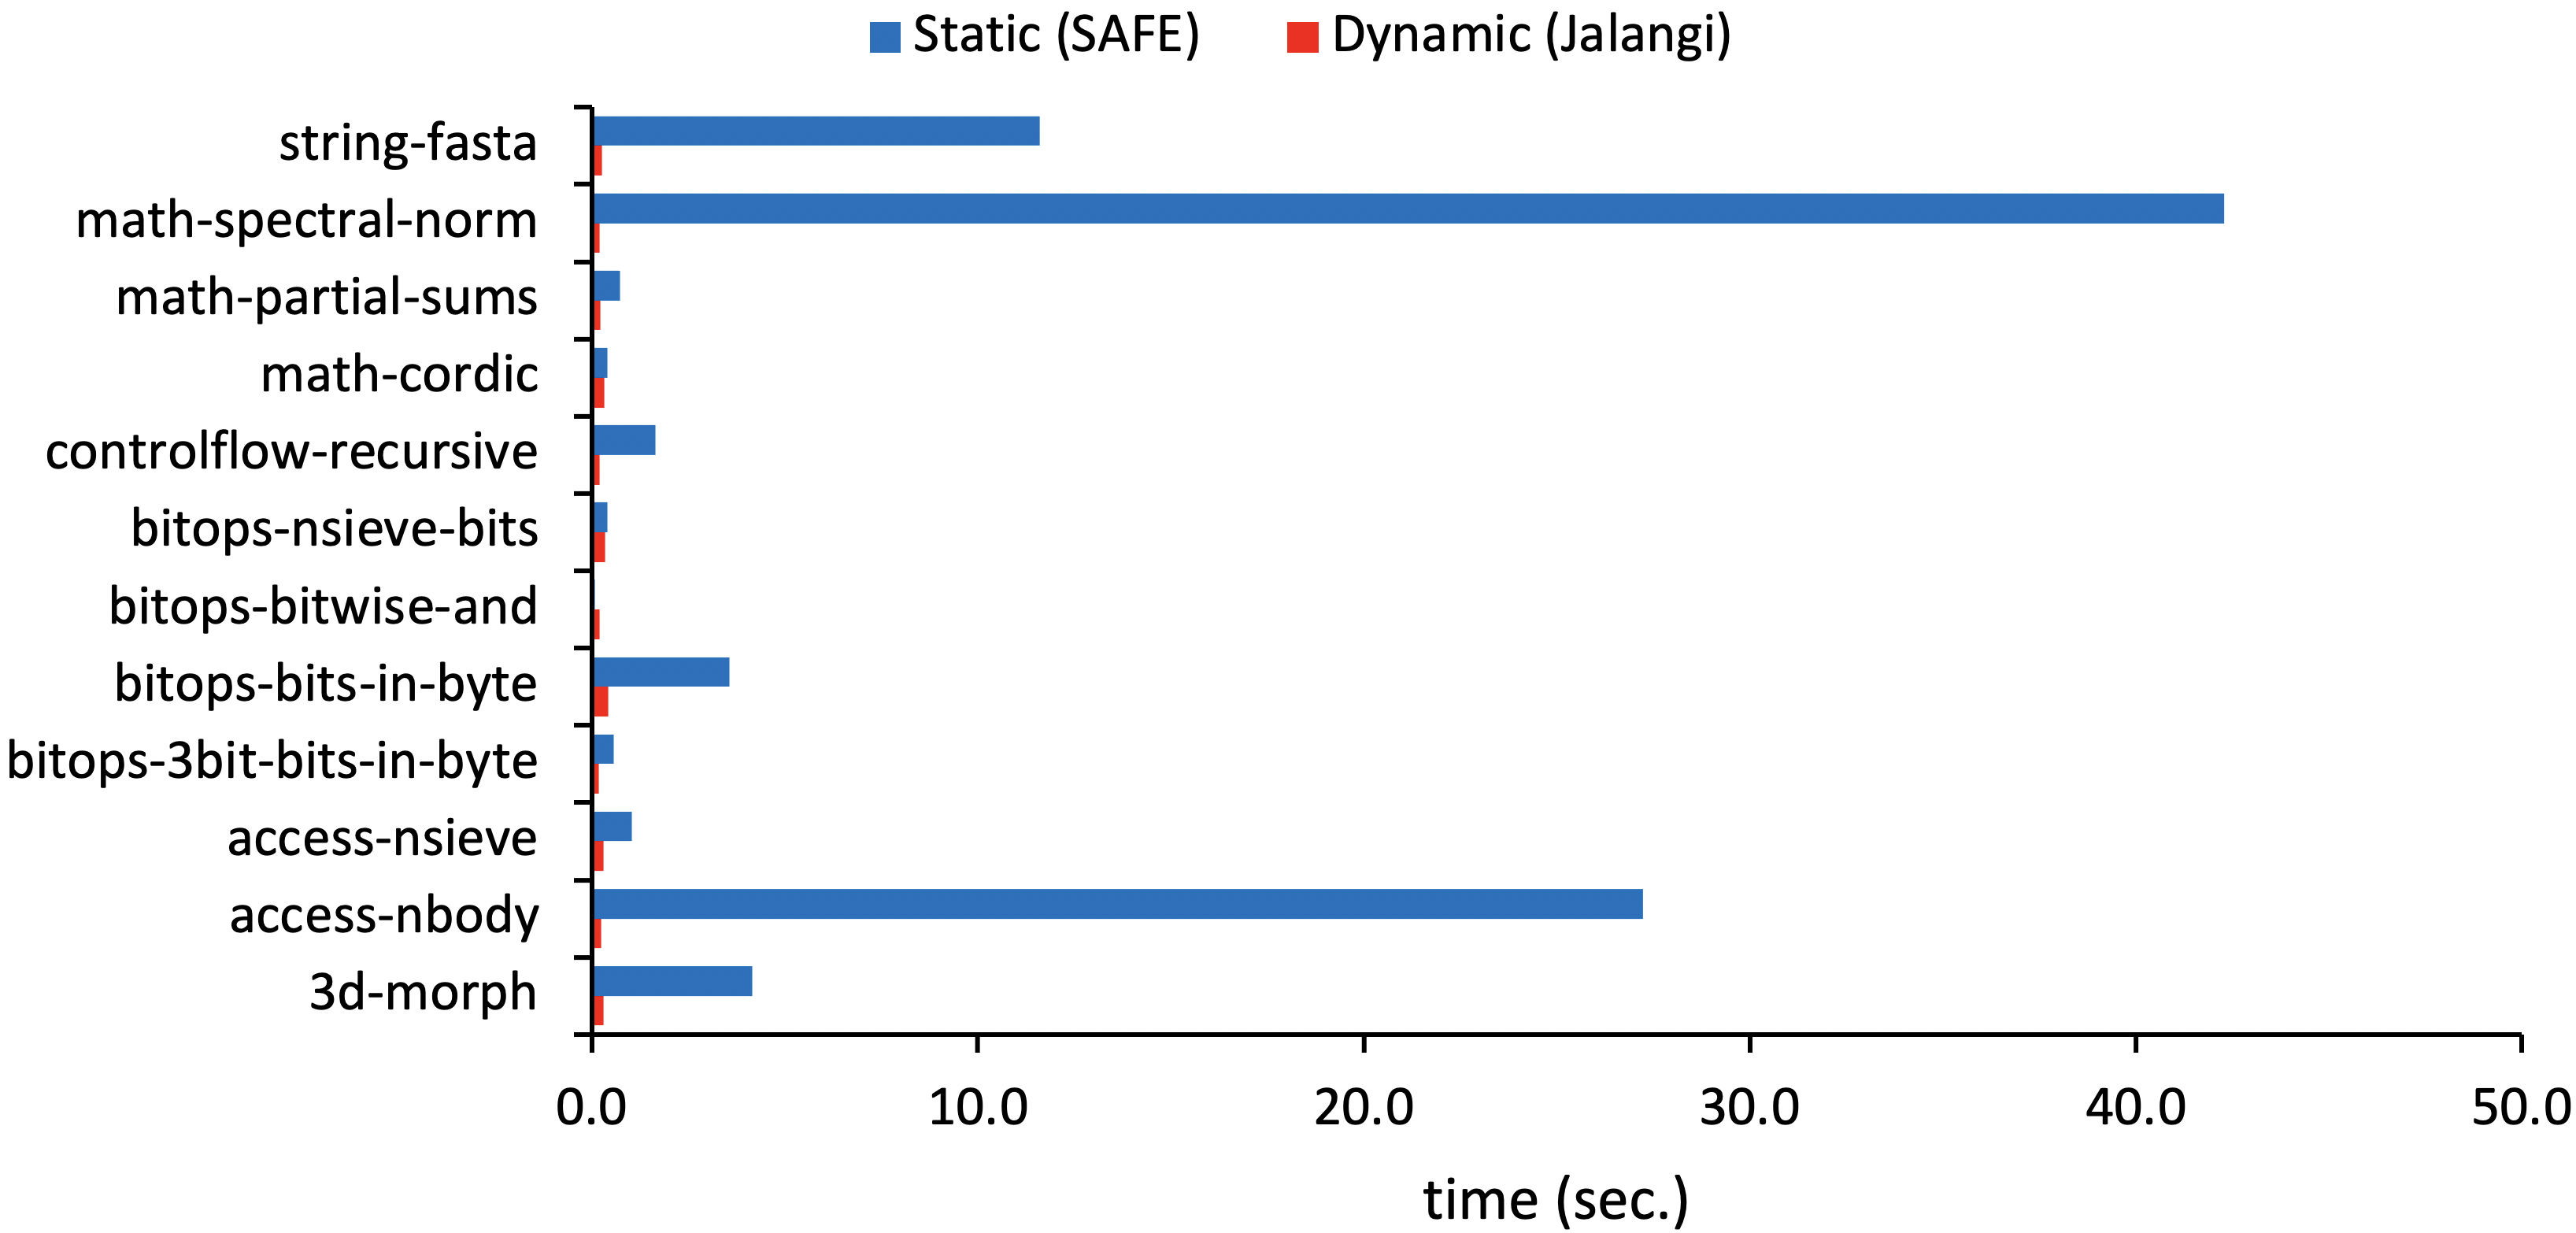
\includegraphics[width=\linewidth]{img/performance_v8v7}
  \vspace*{-2em}
  \caption{Performance of a dynamic analyzer and a static analyzer for a subset
  of the SunSpider benchmark}
  \label{fig:performance}
  \vspace*{-1em}
\end{figure}

To alleviate these problems, researchers have leveraged
dynamic analysis during static analysis.  Because dynamic
analyzers such as Jalangi~\cite{jalangi} and DLint~\cite{dlint} run on
highly-optimized commercial JavaScript engines, they are much faster than
static analyzers.  Figure~\ref{fig:performance} shows that the dynamic analyzer
Jalangi is 34.8x faster than the static analyzer SAFE for a subset of the
SunSpider benchmark.  Using high performance dynamic analysis, researchers have
reduced the scope of static analysis~\cite{determinacy, blendedJS} and constructed
initial abstract states~\cite{battles, eha} and automatic modeling of opaque
code~\cite{sra}.

Unfortunately, existing techniques using dynamic analysis for static analysis
have two limitations: 1) they do not fully utilize the high performance of dynamic
analysis, and 2) they sacrifice the soundness of static analysis.  Most of
them are \textit{staged analyses}, which first extract specific
information via dynamic analysis and utilize it in static analysis.
\citet{determinacy} identify determinate expressions that always have the same
values at given program points, \citet{blendedJS} extract dynamic values to
change expressions to certain literals, and Park et al.~\cite{battles,eha} dump
the initial states of a certain host environment or the entry of an event handler.
However, because they do not utilize dynamic analysis as soon as static
analysis begins, they do not get performance benefits since then.  Moreover,
they sacrifice the soundness of static analysis by performing dynamic analysis.
For example, the SRA model~\cite{sra} uses dynamic analysis for opaque code
with abstract arguments during static analysis.  When the abstract arguments
represent an infinite number of values, it randomly samples finite
concrete values for the abstract arguments, which makes the analysis
result unsound due to missing concrete values.

In this paper, we propose a novel technique to fully utilize
the high performance of dynamic analysis for JavaScript static
analysis in a sound manner by using \textit{dynamic shortcuts}.
During static analysis, one can take a dynamic shortcut, which
consists of three parts: 1) converting the current abstract state to
its corresponding \textit{sealed symbolic state}, 2) performing
\textit{sealed symbolic execution} on the sealed symbolic state, and
3) converting the result of the sealed symbolic execution to its
corresponding abstract state.  Our key observation is that we can use
the fast concrete execution for specific program parts while
preserving the soundness if they do not use abstract values.
For example, consider static analysis of the following code:
\begin{lstlisting}[style=myJSstyle,numbers=none]
    var v = ... // an abstract value
    var obj = { p1: v }, y = "p";
    x = obj[y + 1];
\end{lstlisting}
Because \jscode{y + 1} evaluates to \jscode{"p1"},
the third line assigns the abstract value of \jscode{v} stored in
\jscode{obj.p1} to the variable \jscode{x}.
Note that even though \jscode{obj} contains an abstract value \jscode{v},
because the third line does not ``use'' the value of \jscode{v},
we can concretely execute the code.  Based on this observation,
we introduce sealed symbolic execution, which is concrete execution
using \textit{sealed symbolic values}.  A sealed symbolic value is a
representation of an abstract value in symbolic execution; it signals
the end of the current dynamic shortcut when the sealed symbolic
execution tries to access its value.
To evaluate our technique, we implemented $\tool$ using both SAFE
and Jalangi and analyzed 269 official tests of Lodash 4 library.

The contributions of this paper include the following:
\begin{itemize}
\item We present a novel technique for JavaScript static
analysis to leverage the high performance of dynamic analysis using
dynamic shortcuts.  We formally define the technique and prove
its soundness and termination.
\item We actualize the proposed technique in $\tool$, an
extended combination of SAFE and Jalangi.
\item For empirical evaluation, we analyzed 269 official tests of
Lodash 4 library.  The experiment shows that $\tool$ outperforms
SAFE \inred{X.X}x on average.  Moreover, by using dynamic shortcuts
instead of manual modeling for \inred{XX.X} opaque functions,
$\tool$ improves the analysis precision to detect 5.97 more dead branches on
average.
\end{itemize}

In the remainder of this paper, Section~\ref{sec:motivation} explains the
motivation of this work with a simple example.  Section~\ref{sec:formal}
formalizes the language-agnostic part of the technique in the abstract
interpretation framework.  Then, we extend the formalization with
JavaScript specific features in Section~\ref{sec:javascript}.
Section~\ref{sec:implementation} describes important details of the
$\tool$ implementation.  We explain the evaluation results of $\tool$
with real-world benchmarks in Section~\ref{sec:eval}.
Section~\ref{sec:related} discusses related work and
Section~\ref{sec:conclusion} concludes.
